\documentclass{article}

\usepackage{times}
\usepackage{uist}

\usepackage{graphicx}
\usepackage{caption}
\usepackage{subcaption}

\usepackage{dblfloatfix} 
%\makeatletter
%\let\@copyrightspace\relax
%\makeatother
 
\begin{document}

% --- Copyright notice ---
\conferenceinfo{UIST'12}{October 7-10, 2012, Cambridge, MA, USA}
\CopyrightYear{2012}
\crdata{978-1-xxxx-xxxx-x}

% Uncomment the following line to hide the copyright notice
% \toappear{}
% ------------------------

\bibliographystyle{plain}

\title{Spatial augmented reality to enhance \\
       physical artistic creation.}

%%
%% Note on formatting authors at different institutions, as shown below:
%% Change width arg (currently 7cm) to parbox commands as needed to
%% accommodate widest lines, taking care not to overflow the 17.8cm line width.
%% Add or delete parboxes for additional authors at different institutions. 
%% If additional authors won't fit in one row, you can add a "\\"  at the
%% end of a parbox's closing "}" to have the next parbox start a new row.
%% Be sure NOT to put any blank lines between parbox commands!
%%

\author{
\parbox[t]{9cm}{\centering
	     {\em Jeremy Laviole}\\
	     Univ. Bordeaux, LaBRI,  UMR 5800, F-33400 Talence, France.\\
         CNRS, LaBRI,  UMR 5800, F-33400 Talence, France.\\
	     Inria, F-33400  Talence, France.\\
	     laviole@labri.fr \vspace*{5mm}}
\parbox[t]{9cm}{\centering
	     {\em Martin Hachet}\\
	     Inria, F-33400 Talence, France.\\
	     LaBRI, UMR 5800, F-33400 Talence, France.\\
	     martin.hachet@inria.fr}
	\\
                 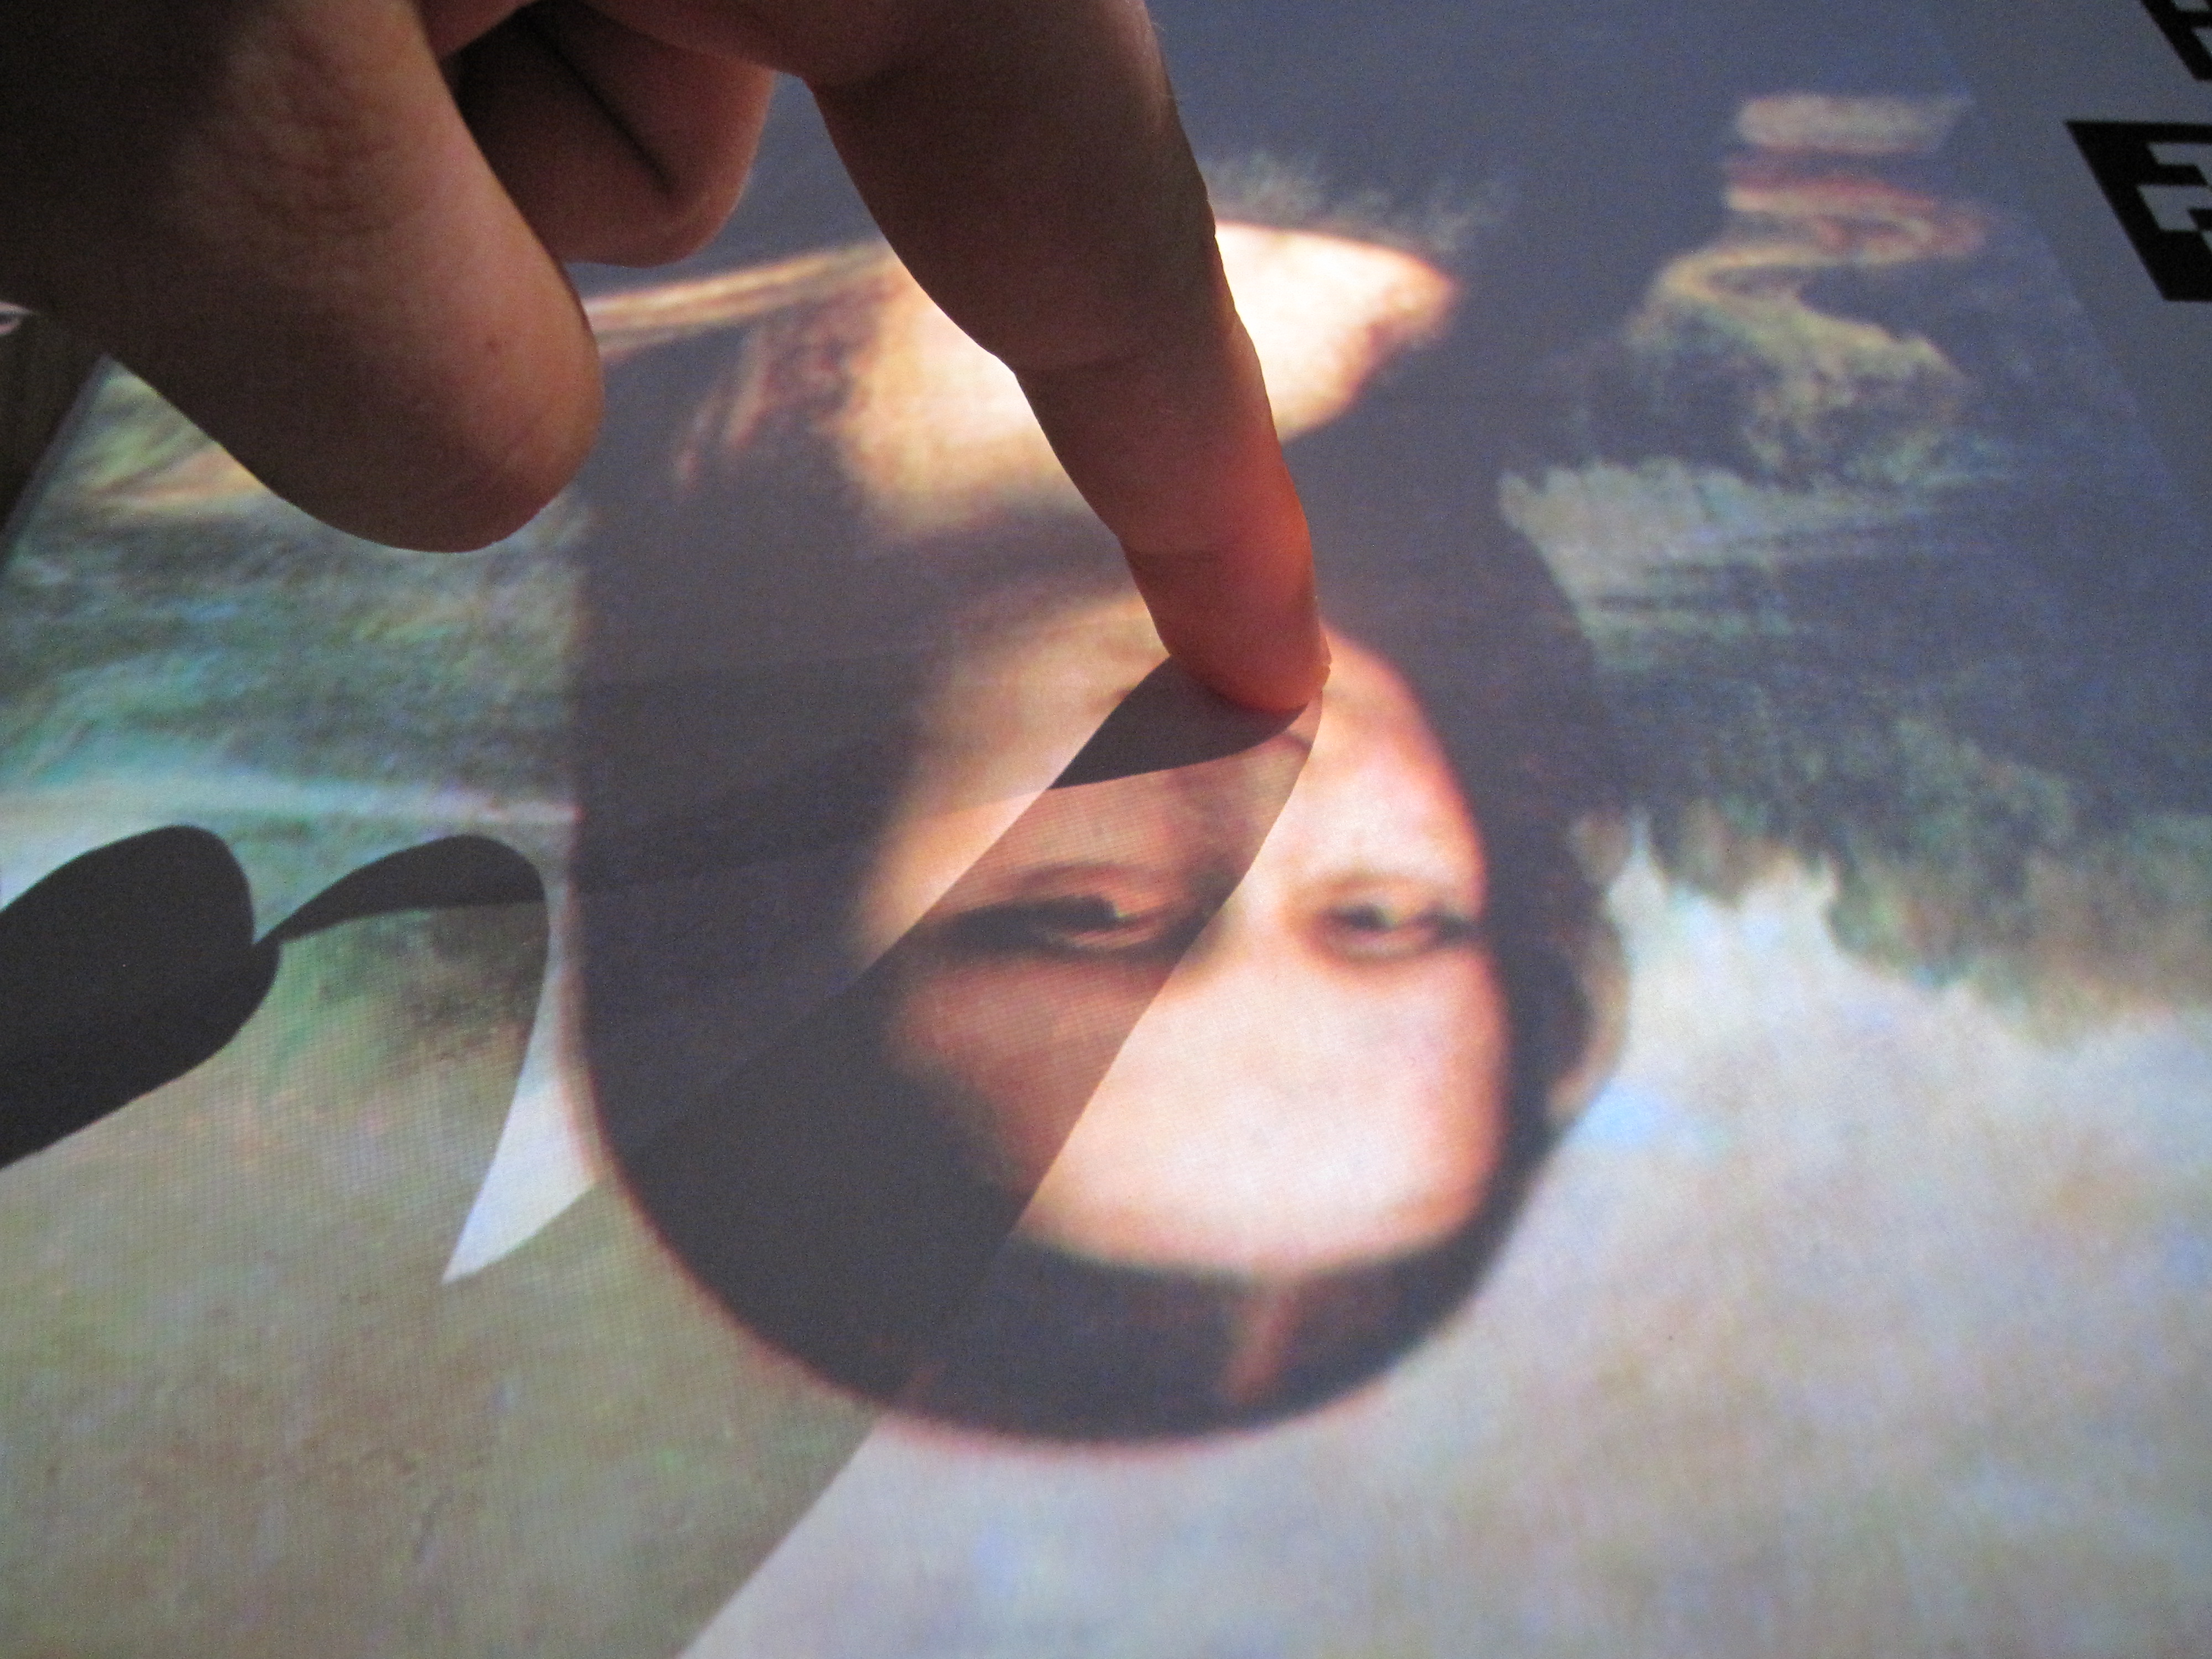
\includegraphics[height=2.5cm]{mona}
               \hspace{0.2cm}     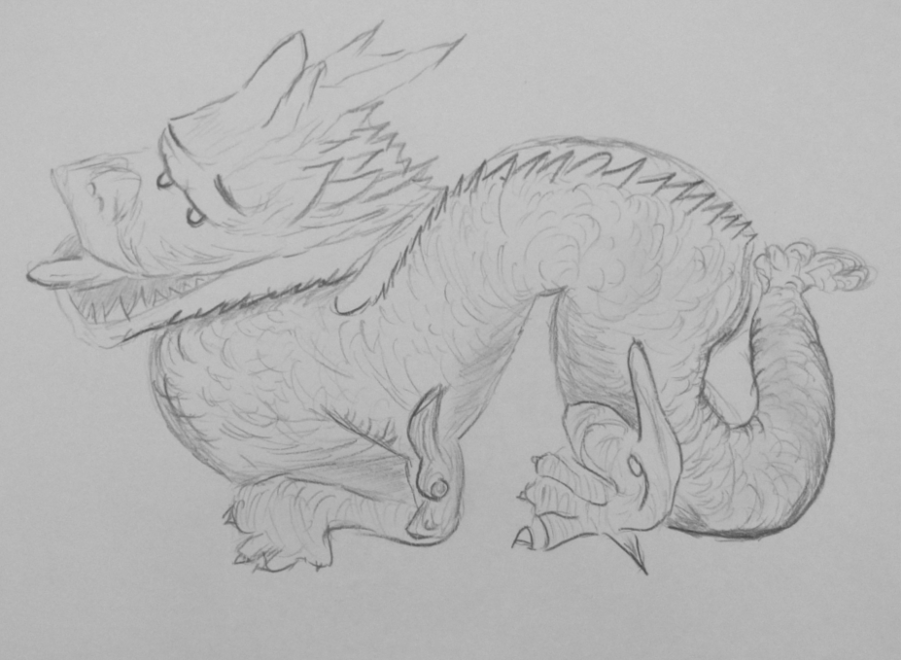
\includegraphics[height=2.5cm]{dragon}
                 \hspace{0.2cm}   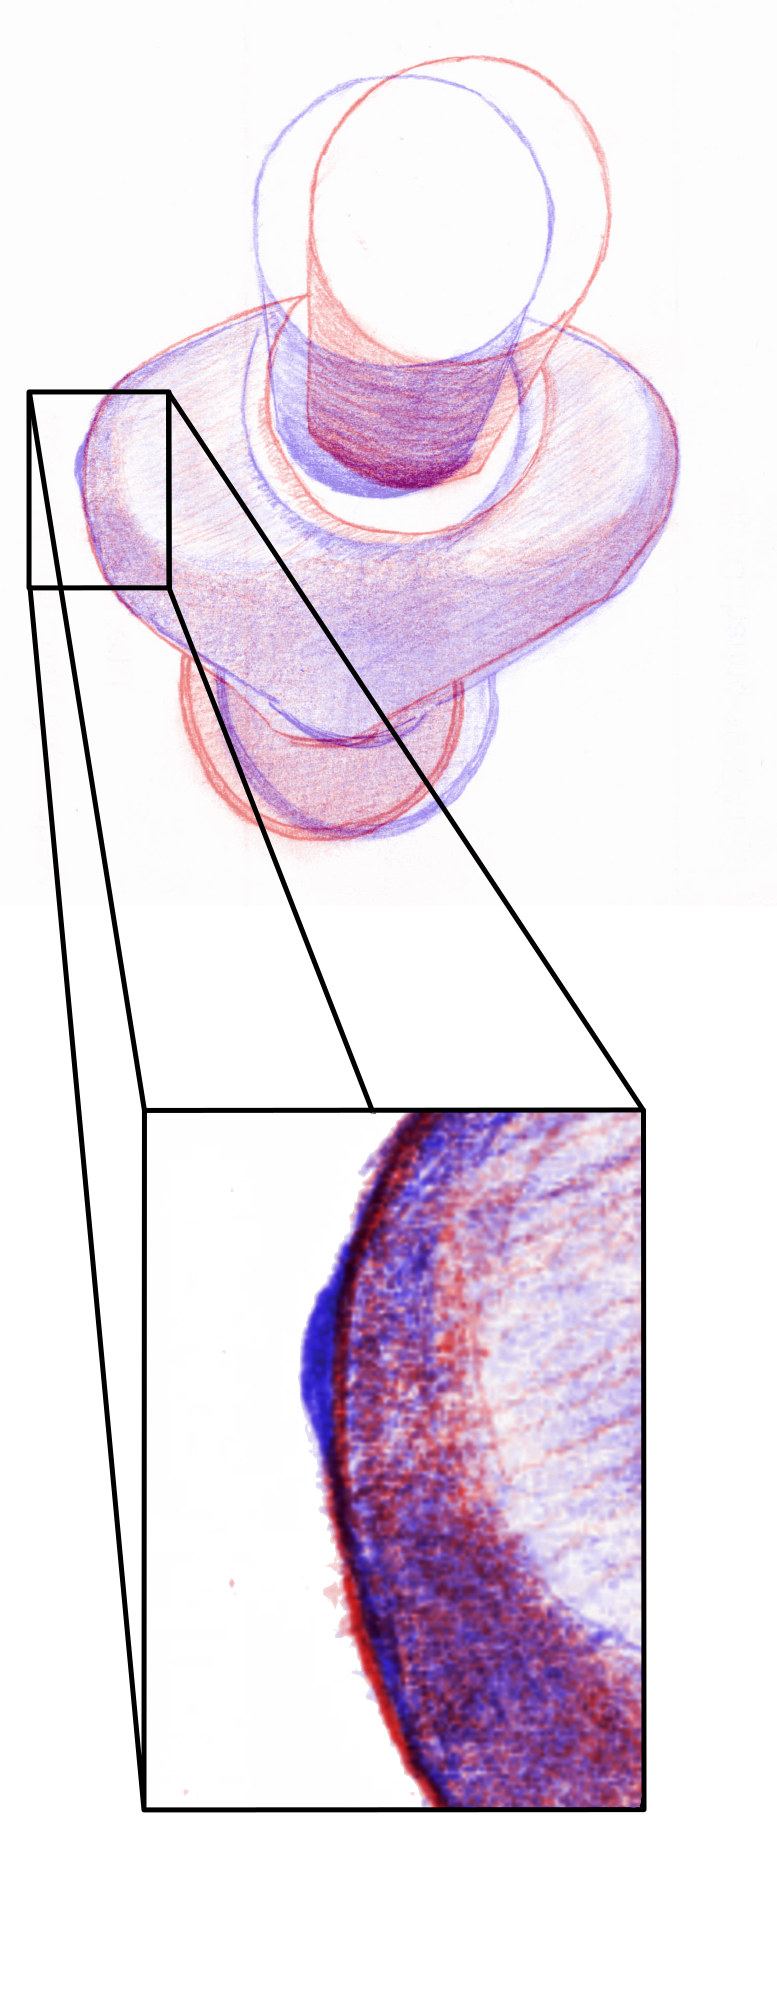
\includegraphics[height=2.5cm]{vase}
                 \hspace{0.2cm}   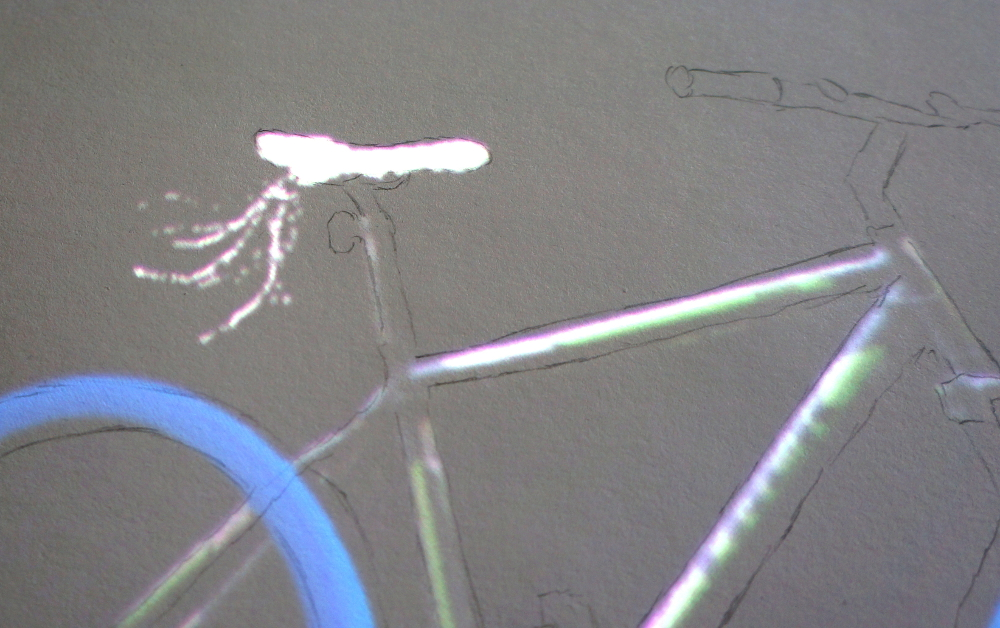
\includegraphics[height=2.5cm]{velo4}
                \hspace{0.2cm}    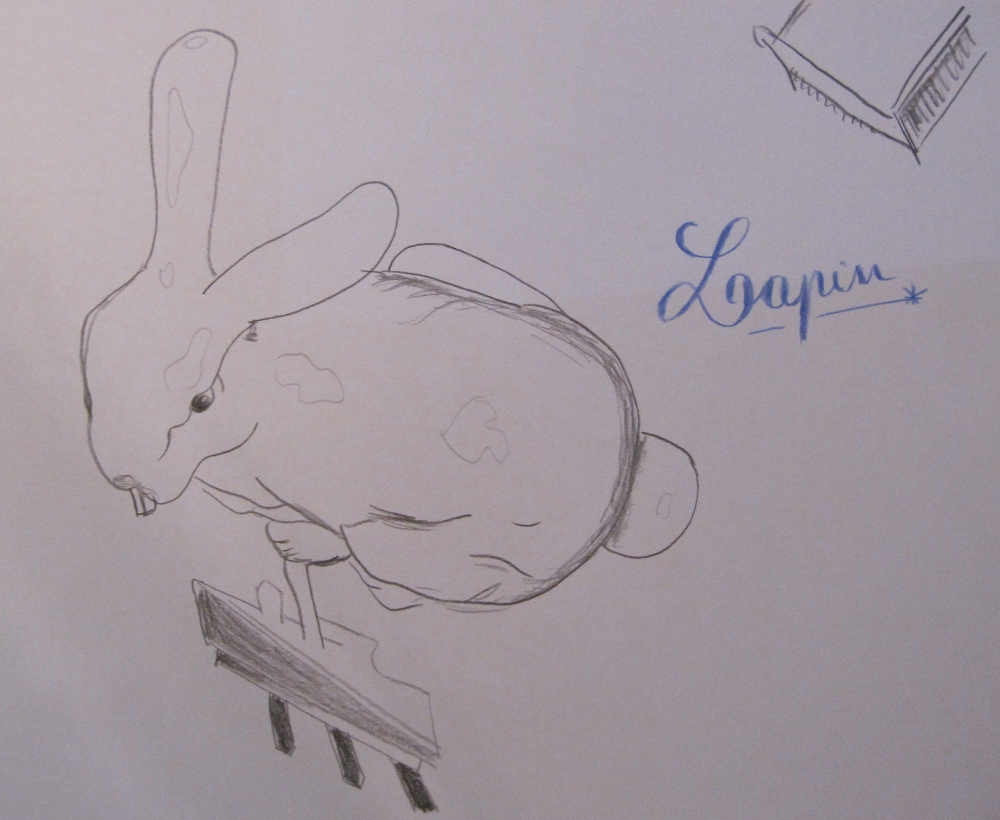
\includegraphics[height=2.5cm]{laapin}  
                \\ \centering \small Left to right bla bla bla.     
}


\maketitle

\abstract

Spatial augmented reality (SAR) promises the integration of digital information 
in the real (physical) world through projection. In this doctoral symposium paper,
I propose different tools to fasten and ease the drawing by projecting photos, 
virtual construction lines and interactive 3D scenes. After describing them, I 
explain some future challenges to explore such as the creation of tools which helps to create 
drawings that are "difficult" to achieve for a human being, but easy to do by a computer. 
Furthermore, I propose some insights for the creation of digital games and programs which 
can take full advantages to have a human and physical constraints.

\classification{H5.2 [Information interfaces and presentation]:
User Interfaces. - Graphical user interfaces.}

\terms{Design, Human Factors (Your general terms must be any of the
  following 16 designated terms: Algorithms, Management, Measurement,
  Documentation, Performance, Design, Economics, Reliability,
  Experimentation, Security, Human Factors, Standardization,
  Languages, Theory, Legal Aspects, Verification. See for more details.)}

\keywords{Spatial augmented reality, user interfaces, fine arts}

\tolerance=400 
  % makes some lines with lots of white space, but 	
  % tends to prevent words from sticking out in the margin

\section{INTRODUCTION}

For a few years now, augmented reality has reached the general public. This is due to the availability 
of webcams in every laptop and mobile phone and software such as ARToolKit~\cite{wagner2007artoolkitplus}.
The augmentations are overlayed on reality and visualized though a screen. 
Even though it is convenient to navigate in the digital world by moving; for many 
applications the users want to have the hands free to interact directly with the 
real world and not by touching a screen. In order to overcome these limitations, the digital information can be projected into reality, this is called spatial augmented reality (SAR)~\cite{raskar1999table}.


In SAR, the visualizations and interactions space are the same; it can create very natural user experiences. Conversely, SAR applications are bounded 
to real-life, thus it is harder to represent data behind real objects because the projection
support will importantly influence the visualization.
Recent work in SAR explore the projection support as the main interaction element. The 
augmented reality part will add new informations, some ideas of applications are described
in \cite{mistry2009sixthsense}. The same idea is explored in \cite{sodhi2012lightguide}, where the projection guides the user's movement. 
In~\cite{wilson2007depth} and~\cite{jones2010build} the freedom of movement of SAR is used to create games which adapts itself to the projection support. Another approach in~\cite{harrison2011omnitouch}, is to use SAR directly on the user's arm or a notepad to control a mobile phone or take notes. \cite{flagg2006projector} Flagg \textit{et. al.} created a SAR application to ease the painting process, they propose tools to help the user to mix fresh paint and to apply the different layers in the right order. 

This kind of SAR in context is very promising, it is a first step for a more natural merge of the digital world and the real world. In order to create applications that fits on the physical world, making it richer and more interactive. In this paper, I state the objectives which led to my past and current works on SAR for drawing. Then, I will conclude with a discussion of the future possibilities such as the integration of physical drawing in digital applications.


% Direction de la th�se pour en r�alit� augment�e. 

\section{Motivations for SAR for physical drawing.}

Coming from a background of computer science specialized in virtual reality and computer graphics, my first desire was to create tools and interactive applications in SAR. More specifically I wanted to use the power of real-time rendering for get an unique man-made creation. 
There are many advantages to create digital drawings instead of physical ones. The most important one, is the possibility to go back and try again; which is obviously impossible in the physical world. I will not list all the possibilities offered by digital drawing, but some of them can be hard to reproduce for physical creation, such as the flexibility of digital layers, the copy/paste operations, filling regions with colors and textures and zooming operations.

Conversely, physical creation allows a direct contact between the artist and the creation. The result will be unique and will contain traces of all the errors corrected. The variety of tools comes from a legacy of thousands of years of artistic creations. Each pen or paint has its own smell and behaviour on the paper and tactile feeling. The bound between the artist, its tools and the resulting creation has history: from the acquisition of tools, to the whole creation process to achieve the desired result, or not. This bound may be different from digital creation, the choice of a digital brush or effect will not have any cost, and will generally not require to move from the computer. 




%My main motivation is to create tools to make the creation and drawing process easier, faster, and for better results. Furthermore, I would like to push the possibilities of physical drawing; enabling drawing creations that are hard to imagine or visualize for a human such as stereoscopic drawings.

In order to use the possibilities of real-time rendering, the artist will need to visualize and modify a 3D scene. In the next section, I present the system I created enabling projection on interactive paper sheets, allowing the projection of photos to interactive 3D scenes. 


\begin{figure}[!tb]
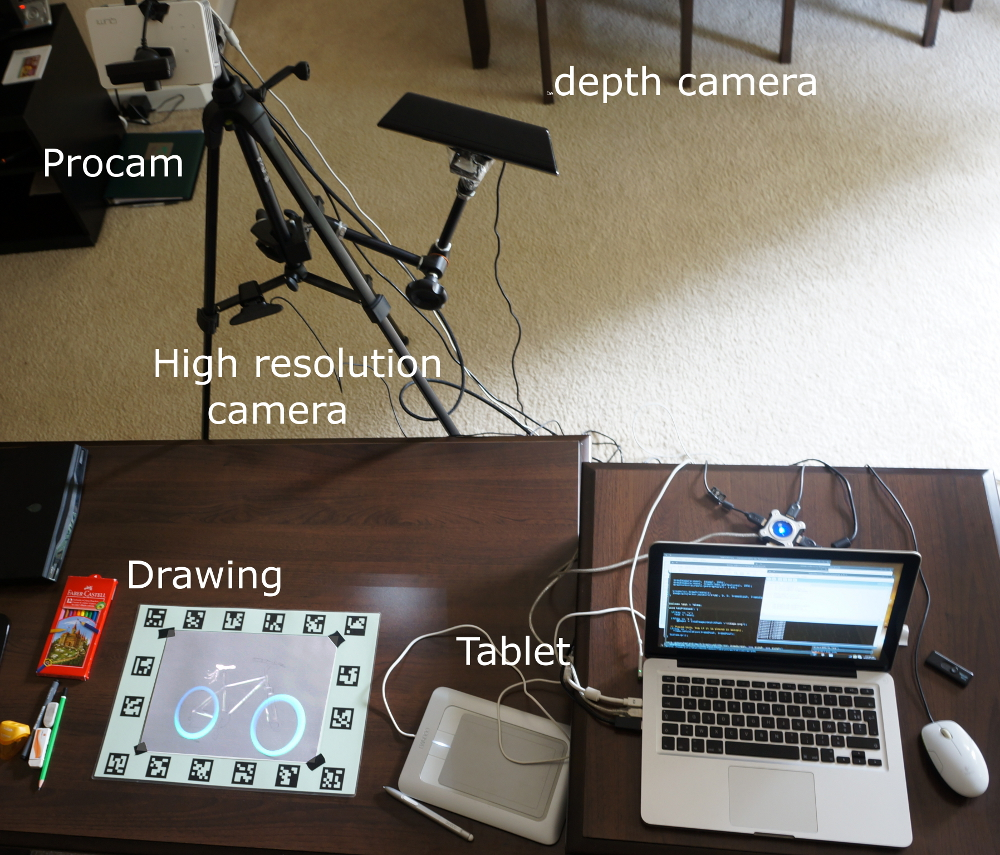
\includegraphics[width = 85mm]{DSC00299-2-rogne-annote.JPG}
\caption{View of the system in a home configuration. The whole sensing and projecting system is mounted on a tripod, making it easily transportable.} 
\label{fig:system}
\end{figure}


\section{Spatial augmented reality and interactivity}

\subsection*{The system}

For the creation of the system, we wanted to have as less constraints as possible: no constraint on the creation tools nor on the support. More importantly, we wanted to keep a large freedom of movement. Consequently, the system does not add any constraint to the traditional setup, and seamlessly integrate the digital elements within it. 

The hardware system is composed of a small projector-camera (procam) set, and a depth camera, as seen in Figure~\ref{fig:system}. We chose overhead projection to enable any support, and we use the depth camera to make the system interactive. The user interface is composed of tracked paper sheets, one or more is dedicated to the creation space. The paper or canvas is surrounded by markers to achieve a high precision detection of its position. The whole drawing area is made tactile by the depth depth camera, even allowing 3D pointing interactions over it. Another paper sheet is used for the user interface, generally containing virtual buttons.


The goal of the system is to achieve a high speed tracking and more importantly high fidelity projection. As the tracking speed may make the system less appealing or slow the user, a bad calibration will make it unusable. The capture and projection process requires a precise calibration to achieve the desired results. 
The hardware used is widely available for a moderate cost, the projector used is a DLP LED projector, the camera and depth camera are video game console accessories. 
 
 


\subsection*{3D projection and manipulation}

The firsts experiments involved the projection of photos inside the tracked paper sheet. The task was to create a drawing from the projected image, the projection acts as tracing paper. Some results are presented in Figure~\ref{fig:lyspanda}. From these experiments, we had some user feedback; the tracking does not have to be fast during the drawing phase: when the user moves the drawing support, he or she can wait a second or two before drawing again. Another point is that any shift between the projection and the drawing will make the drawing much harder, and less comfortable. We also included tools to change the intensity of the projection, which was necessary to add any details to the drawings. 

\begin{figure}[!h]
        \begin{subfigure}[b]{0.20\textwidth}
                \centering
                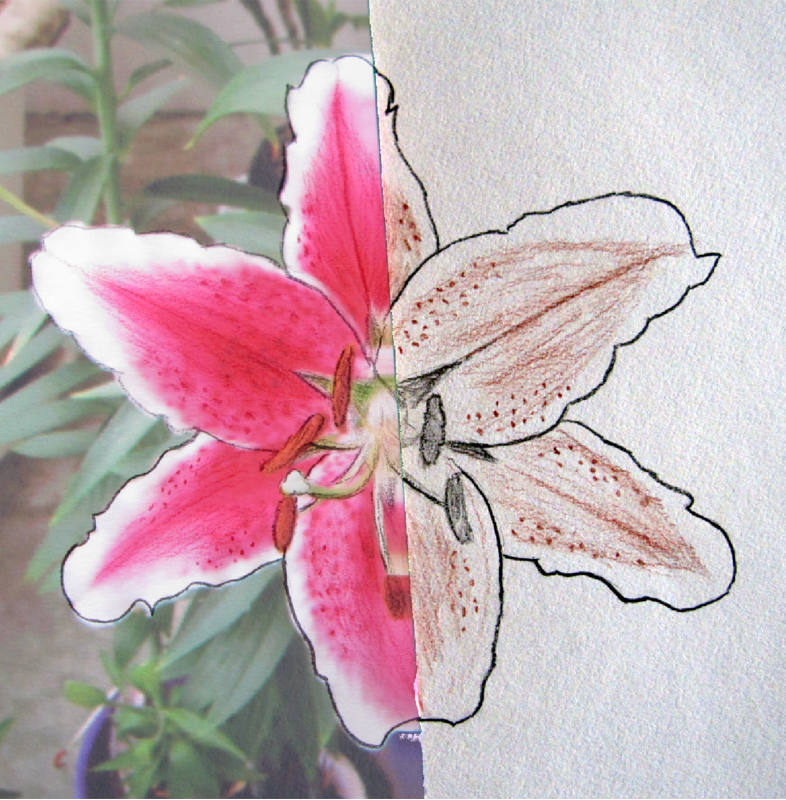
\includegraphics[height=3.2cm]{lys}
                \caption{A lily flower.}
                \label{fig:lys}
        \end{subfigure}%
        ~ %add desired spacing between images, e. g. ~, \quad, \qquad etc. 
          %(or a blank line to force the subfigure onto a new line)
        \begin{subfigure}[b]{0.25\textwidth}
                \centering
                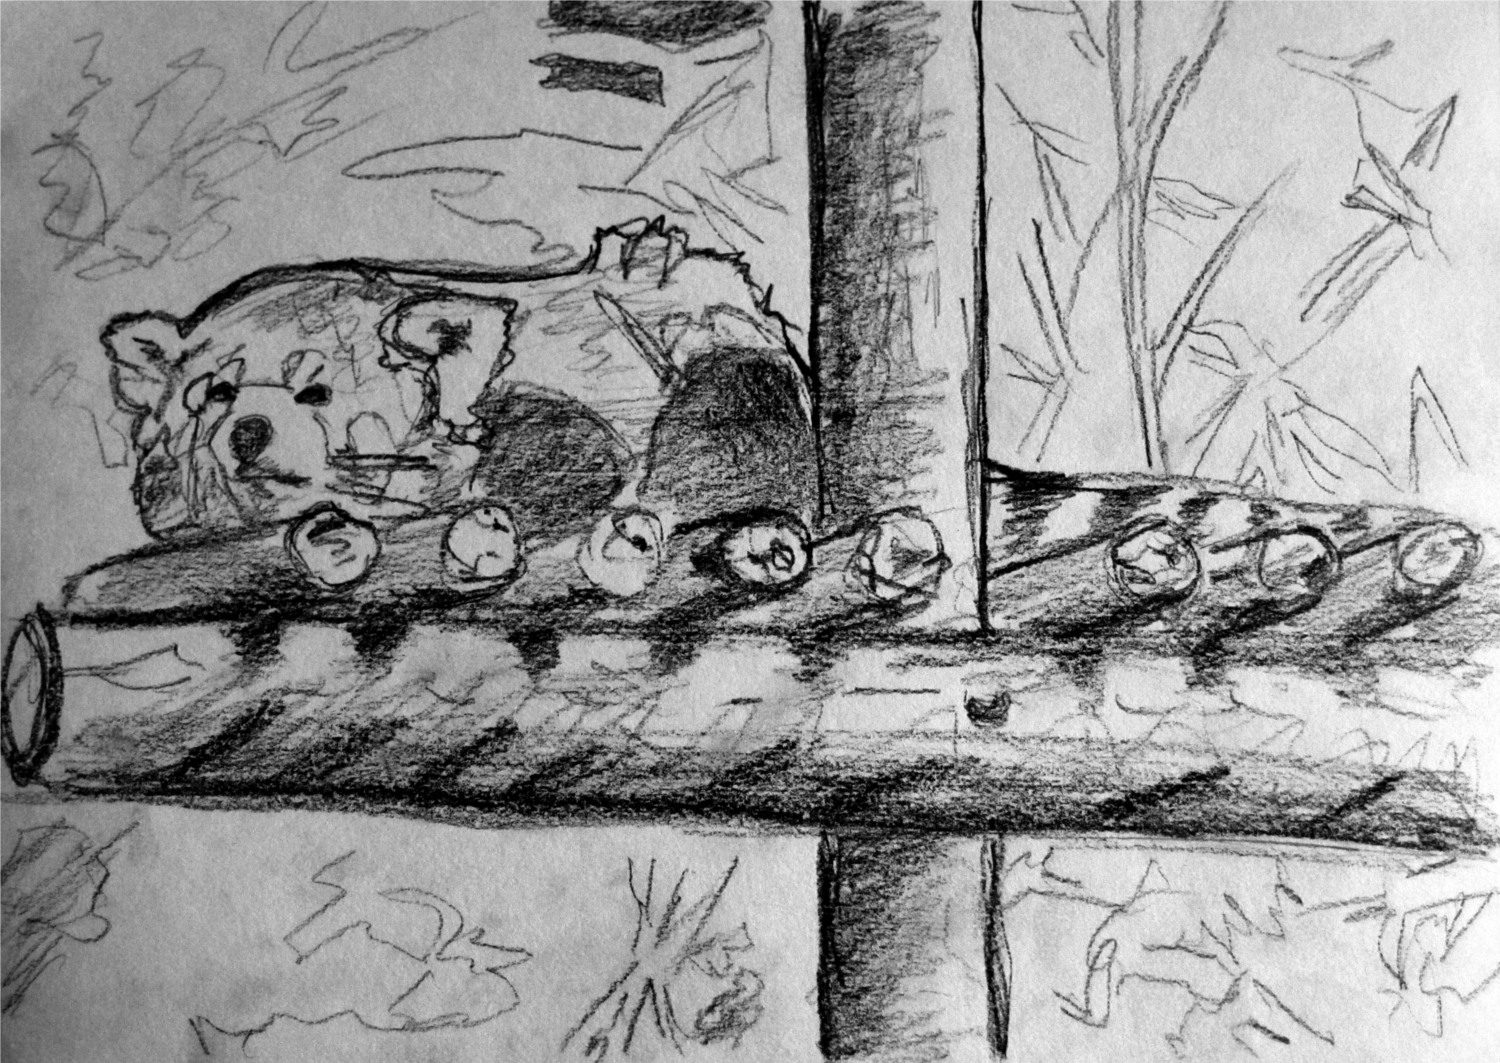
\includegraphics[height=3.2cm]{panda}
                \caption{A red panda.}
                \label{fig:panda}
        \end{subfigure}
        \caption{The projection of photos on the tracked paper sheet is a comfortable and easy way to create drawings.}\label{fig:lyspanda}
\end{figure}


The second application we developed allows the projection of a 3D scene. A 3D object is projected onto the paper sheet and behaves as if it was directly on the paper sheet. Consequently, if you see the front and want to see the back of the object, you just need to turn the paper sheet on the table. We also included rotate, scale and translate operations using the touch interface, allowing an easier modification of the scene. The point of view of scene is set to the user's head position, but generally we fixed it to make the system more robust and to keep it cheap. The 3D pointing was used to set a virtual light inside the virtual scene. The tangible interface and light placement enhance the perception of the 3D objects. We pushed it further by adding stereoscopic rendering. Using this system, we created an application and a drawing scenario for a general public exhibition in Paris. 


\begin{figure}[!h]
        \begin{subfigure}[b]{0.23\textwidth}
                \centering
                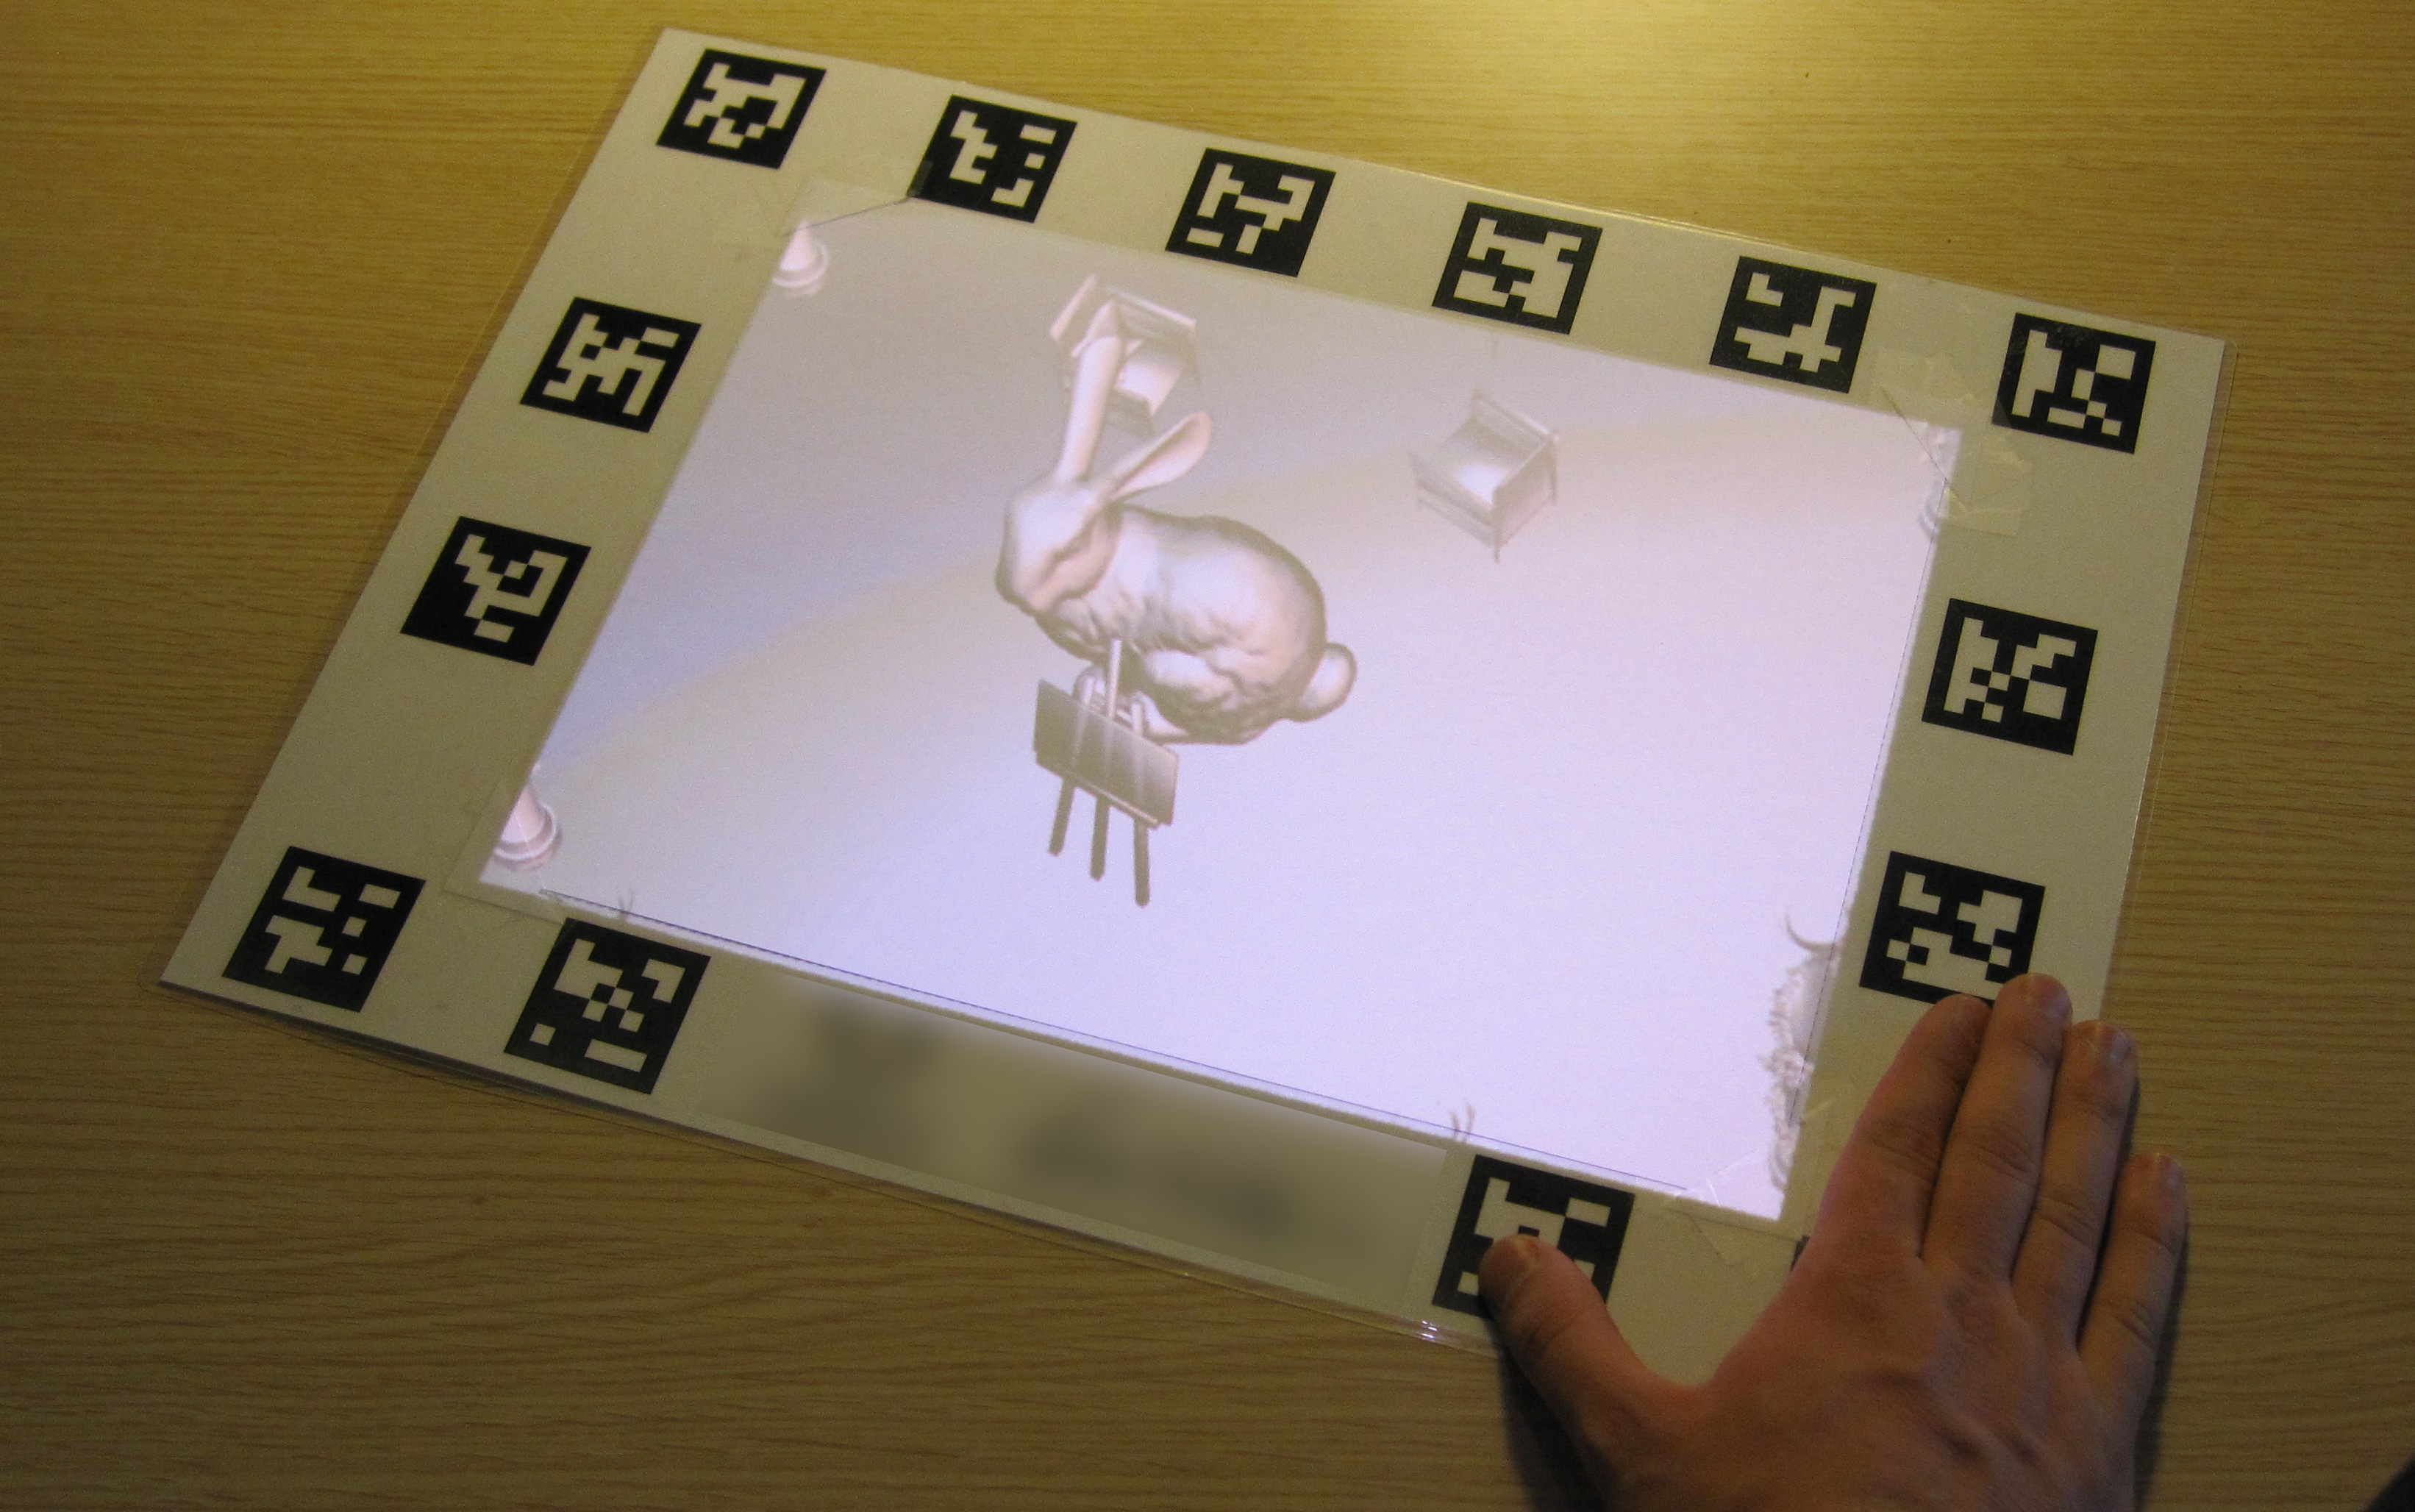
\includegraphics[width=3.9cm]{proj1}
                \caption{Before rotation}
                \label{fig:lapin1}
        \end{subfigure}
        ~ %add desired spacing between images, e. g. ~, \quad, \qquad etc. 
          %(or a blank line to force the subfigure onto a new line)
        \begin{subfigure}[b]{0.23\textwidth}
                \centering
                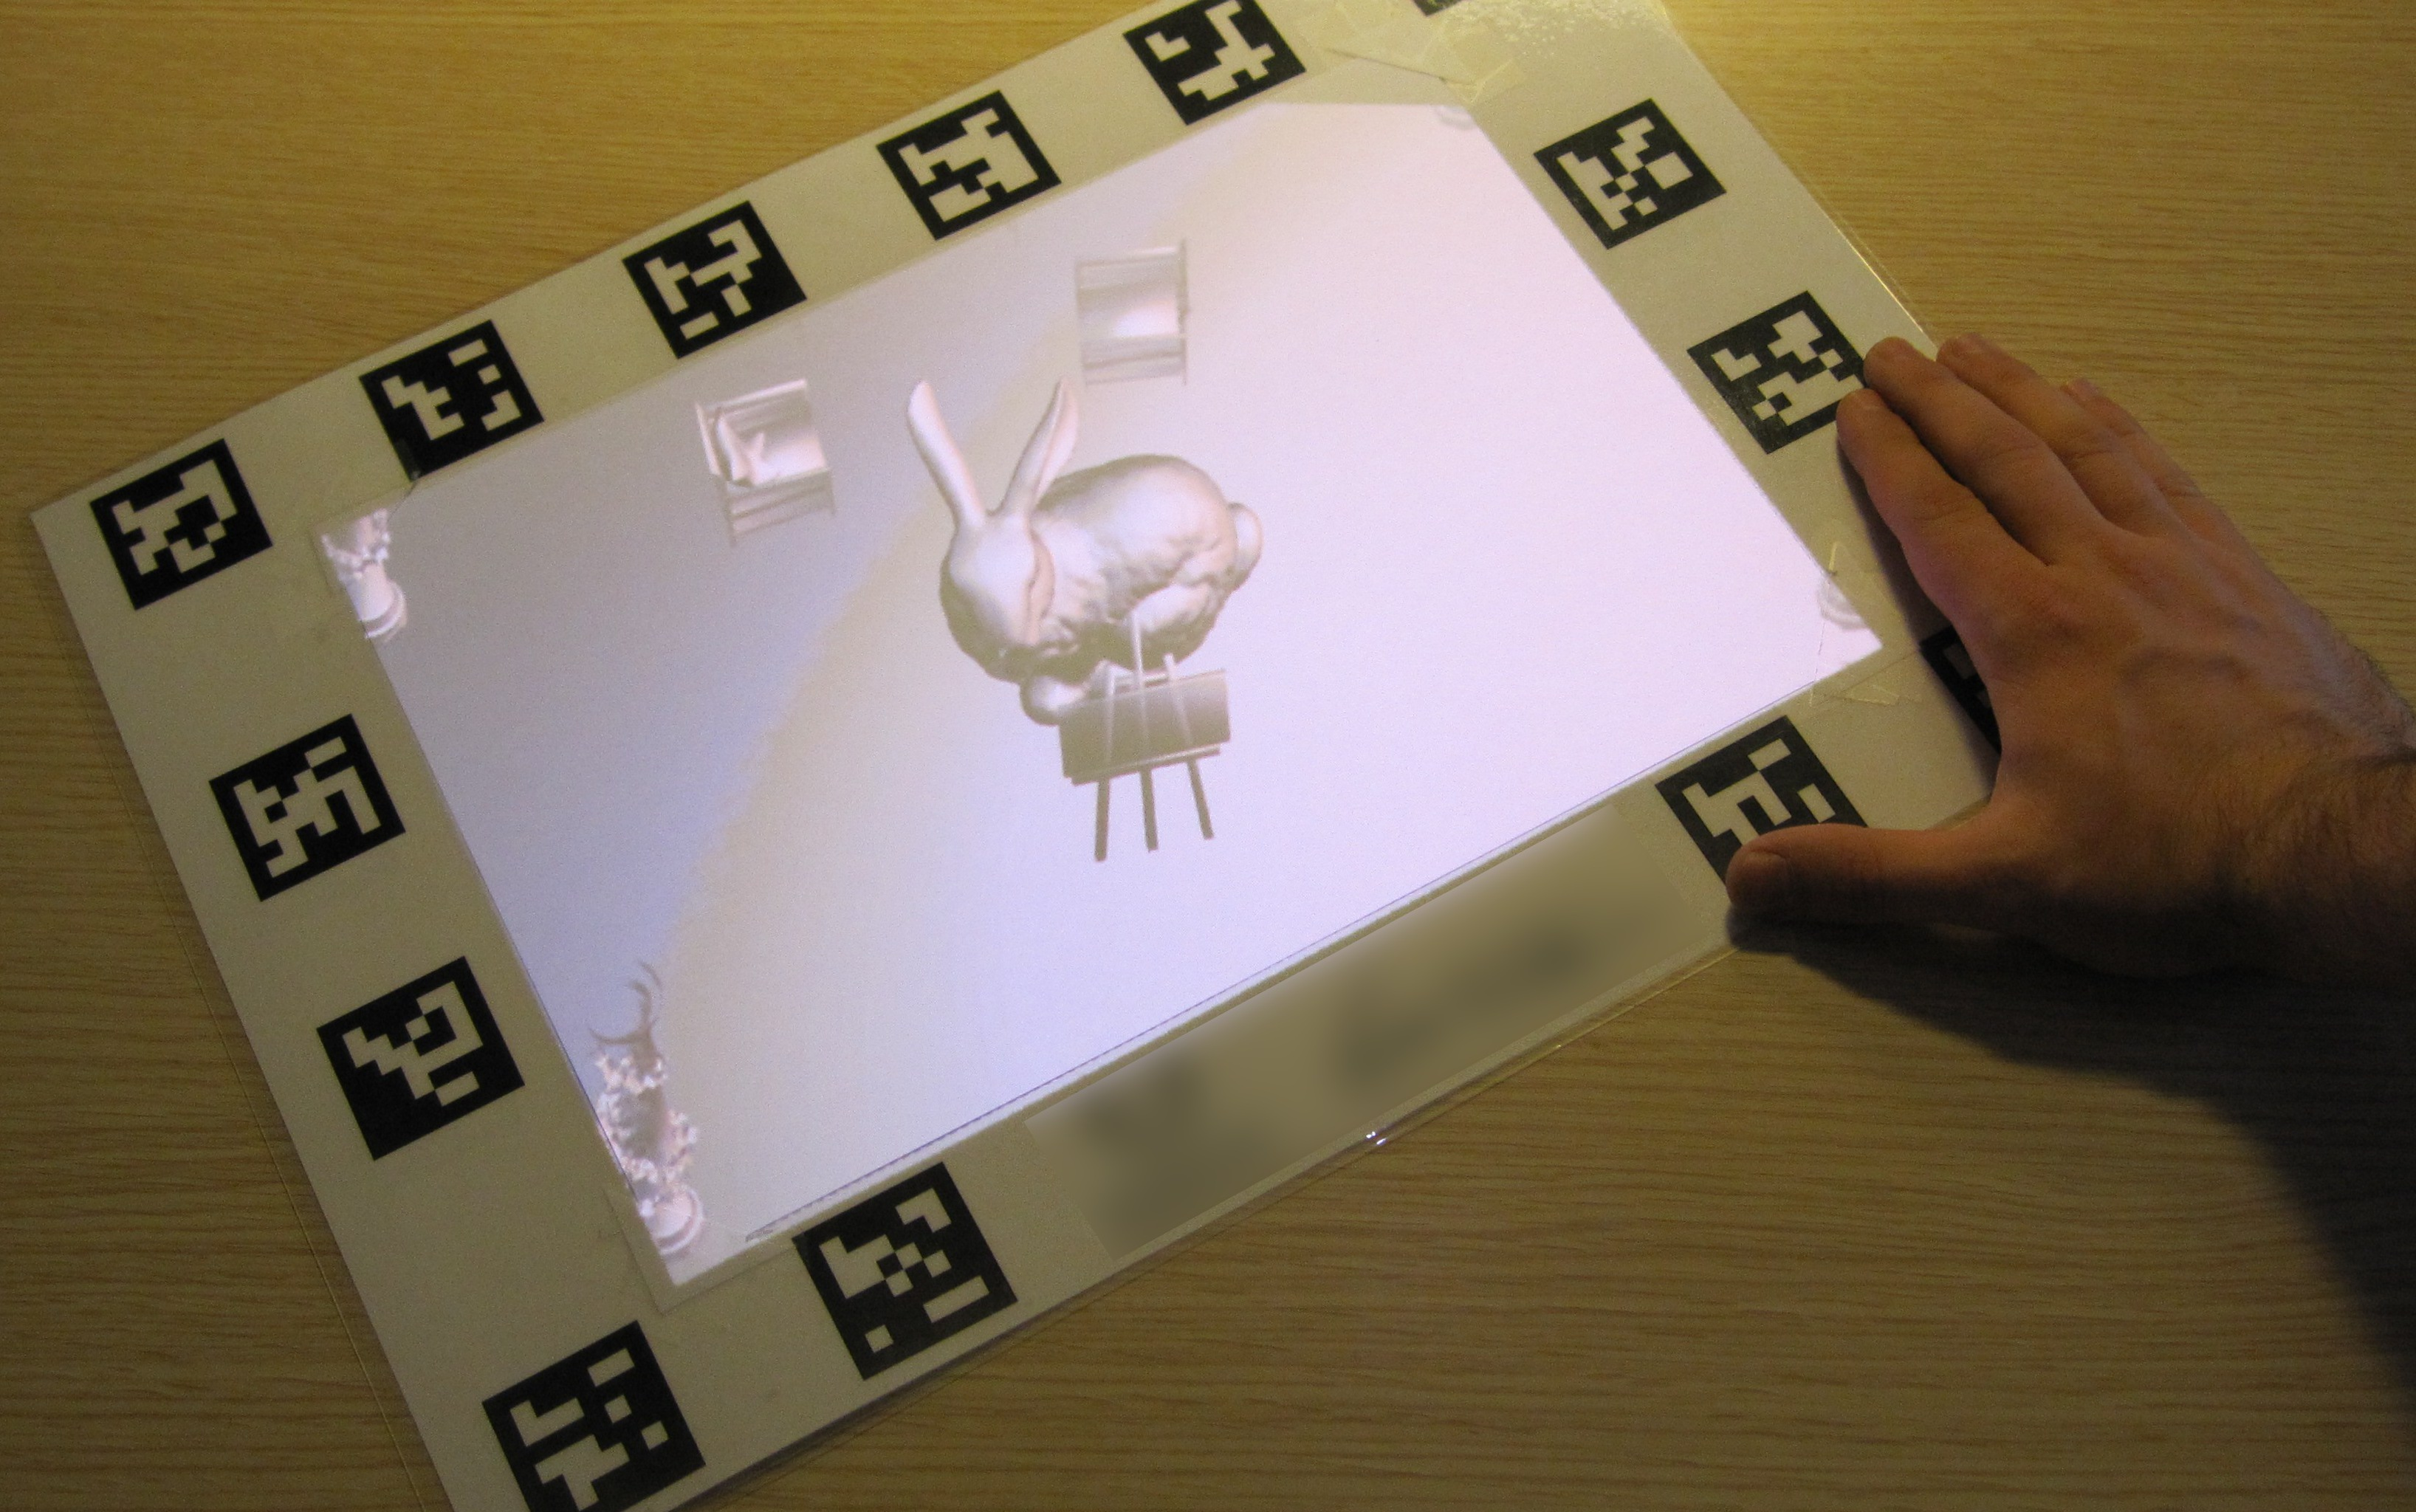
\includegraphics[width=3.9cm]{proj2}
                \caption{After rotation}
                \label{fig:lapin2}
        \end{subfigure}
        \caption{The paper sheet is used a a tangible interface. While its moving, the rendering adapts the view to the new location.}\label{fig:lapins1}
\end{figure}

\subsection*{General public exhibition}

The exhibition lasted more than 3 month, and we were demonstrating and experimenting for more than 12 days. The aim of the demonstration was to explain our research to the general public and to let the visitors experiment. We designed a drawing application using the projection of the 3D scene. We could explain the current challenges of visualization and manipulation of virtual objects. After describing our system and solutions, we could make a quick drawing and let a visitor do another one while answering the questions.

In order to speed up the drawing phase, we used a simple toon shading for the rendering of the scene and a 3D model which was simple to draw, as illustrated in Figure~\ref{fig:3lapins}. The whole description of the system and elements of the presentation were done only using the touch and tangible interface; the mouse, keyboard and screen of the computer were hidden from the visitors.

 
The reception of the general public was good, and seemed magical for some visitors. When the paper sheets are on the table, the system is interactive, but without any paper sheet it is just a table with a few pencil and an eraser. We tested our drawing system nearly on 200 visitors, and nearly every one of them was impressed by the quality of their own drawing. 


\begin{figure}[!h]
\centering
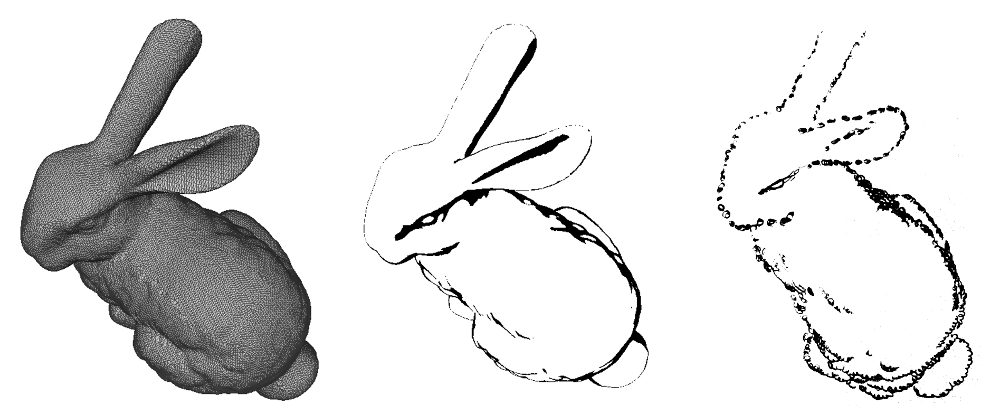
\includegraphics[width=85mm]{108079240.png}
\caption{Illustration of the drawing process. A 3D model is rendered using toon shading and projected. On the right is the resulting drawing.}
\label{fig:3lapins}
\end{figure}



\section{Pushing the limits of drawing}


The first hard drawing I explored with this is stereoscopic drawing. Since recently, stereoscopic screens are widely available, and "3D" movies are getting more and more common. The creation of stereoscopic drawing is hard and repetitive: two nearly identical drawings have to be made. Moreover, the visualization of these drawings require training for free view techniques or more generally a stereoscope. In~\cite{laviole:hal-00671361}, we proposed a tool to create stereoscopic drawings from a pair of generated images. The images are created using the hardware and software described above. 

Just like any drawing, stereoscopic drawings require editions and adjustments. But unlike any drawing, it has to be done twice, and the differences between the two drawings will influence the depth perception of the result. We also included the possibility to take an image of each drawing in order to have an anaglyph preview of the result. 

These experiments have raised many questions and observations. The first observation is on the quality of the drawing: the depth perception will be more influenced by the quality of the shading than by the left/right disparity. We are not sure that two drawings will be required, this question is more personal. If just one drawing is done, and the second one is only the changed elements for stereoscopy, the objective to enhance the real world is not achieved any more: a digital reconstruction is required to visualize the result. 


\begin{figure}[!h]
        \begin{subfigure}[b]{0.23\textwidth}
                \centering
                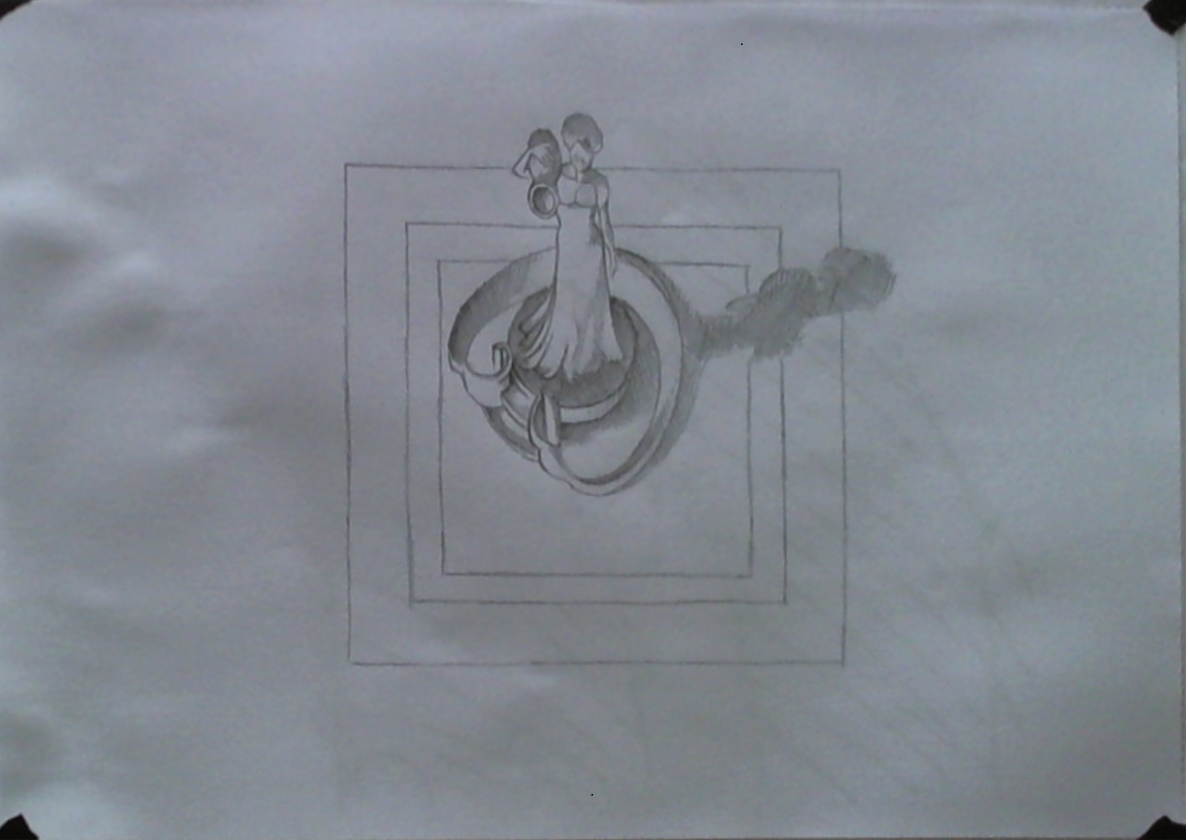
\includegraphics[width=3.9cm]{stereo1}
                \caption{Left view}
                \label{fig:stereo1}
        \end{subfigure}
        ~ %add desired spacing between images, e. g. ~, \quad, \qquad etc. 
          %(or a blank line to force the subfigure onto a new line)
        \begin{subfigure}[b]{0.23\textwidth}
                \centering
                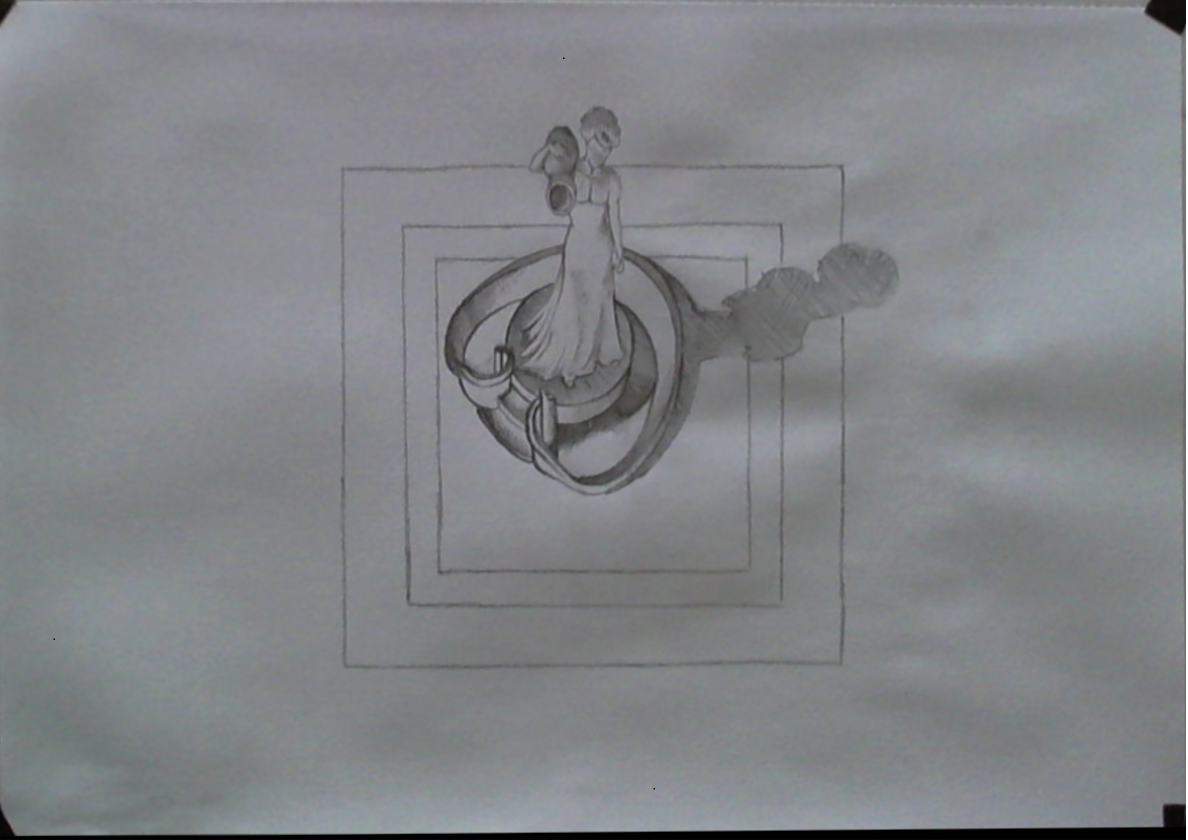
\includegraphics[width=3.9cm]{stereo2}
                \caption{Right view}
                \label{fig:stereo2}
        \end{subfigure}
        \caption{Stereographic pair of drawings.}\label{fig:stereo}
\end{figure}

\section{Perspectives of SAR for drawing}

\subsection*{Interaction techniques}

The inputs and interaction techniques described above allows direct and natural interactions. But, it is not precise for selection and manipulation of the digital information. In order to complement 
these we added a highly precise tablet input (wacom); it allows to overlay digital drawing over the physical one. We also included the possibility to capture the drawing. This way, the drawing itself can be considered as in input method, like in~\cite{hagbi2009shape}. 

\subsection*{New forms of creation}

From our first experiments, most of the users really liked the result of the mix between the real drawing and the projection. The real drawing generally makes the contour stronger and represent the interesting features of the image; while the projection provide complex texture and colors that are very hard to draw. From these, we could allow the creation of hybrid drawings, partly physical and partly digital, a simple example illustrate this in Figure~\ref{velo} The physical drawing may keep blank or less intense parts allowing the projection. The projected elements, unlike drawn elements can contain animations, which enables an interactive exploration of the drawing, or animated drawings. 

\begin{figure}[!h]
\centering
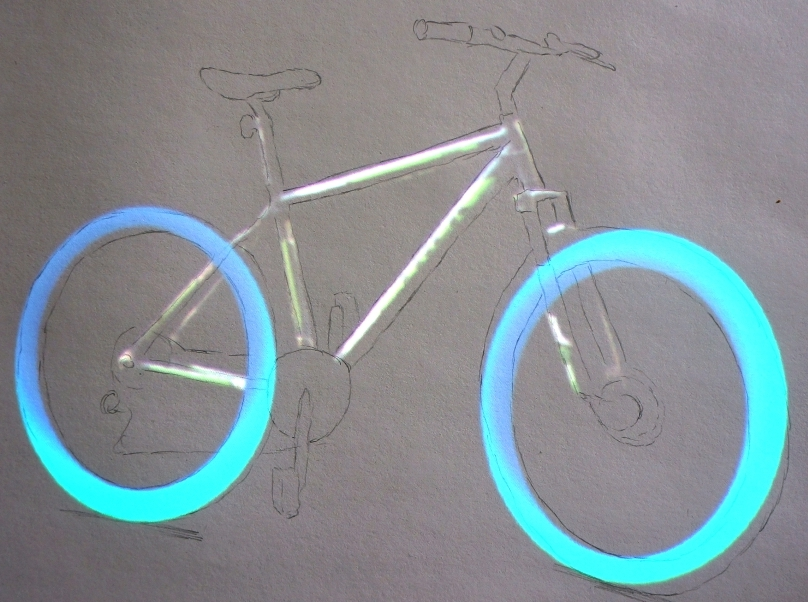
\includegraphics[width=65mm]{velo2}
\caption{Photo of a mix between a physical drawing, real colors from a photo and extra colors added using an image edition software.}
\label{fig:velo}
\end{figure}


\subsection*{Digital games applications}

The fact that a drawing leaves a trace, takes time and can contain errors makes it a good candidates for game creations. An example of games is real-time strategy games. Instead of just putting buildings using the mouse, the player could draw each building. Using more or less symbols to represent each non-moving units. The quality of the drawing could be evaluated to set its properties. The drawing process takes times, and the fact that the quality of the drawing is implied in the game will force to user to make choices on quality or speed. The limitations will not be game limitations, but also player limitations. 
The difficulty levels could imply new drawing skills, such as special shading techniques, or high speed drawing; thus creating a pedagogical game on drawing. 

One could also create construction games, such as Sim City. Instead of creating a digital city, the city maps is drawn directly on the paper, and virtual citizens could come and create their own houses. As described above, the creation of special building could be man-made, and it will create another dimension of the game. The player will think twice when placing the schools and fire station, because moving them will require real time and effort. 

\section{Extensions}

Most of the applications described here are far from using advanced computer graphics techniques. However, some recent works such as ShadowDraw~\cite{leeshadowdraw} shows a desire of the computer graphics community to get closer to the physical world. we could imagine tools assisting the creation of multi-perspective drawings or complex anamorphosis. These kind of drawings require a wide variety of skills that could be compensated by programs. 

Another natural extension, would be the use of the capture and reprojection for the creation of traditional animation. It would be a compelling challenge to take advantage of the digital animation tools, and port them to be used for physical images. 

We proposed some tools to draw 3D objects. An interesting, though difficult approach would be to use multiple drawings to interactively construct a 3D model. The first creations of the designers are generally on paper, and they are multiple view of the objects. It makes them a perfect candidate for interactive reconstruction of the imagined 3D object. This way the designer may create more drawings, and achieve a better inner representation of the object.  

% anamorphose - modelisation 3D - multiperspective

\section{Conclusion}

In this paper I summed up the most interesting work and thoughts of nearly two years of work. The creation of the SAR installation required the acquisition of new knowledge from computer vision and computer graphics. The possibilities with this kind of installation are just starting to be explored. The creation of each application rose many questions touching the fields of computer vision, human perception, computer graphics and challenging design choices. We proposed solutions to ease the drawing, and had the possibility to try them with the general public. 

\bibliographystyle{abbrv}
\bibliography{paper}

\end{document}
